\documentclass[11pt,a4paper]{scrartcl}
\usepackage[utf8]{inputenc}
\usepackage[german]{babel}
\usepackage{amsmath}
\usepackage{amsfonts}
\usepackage{amssymb}
\usepackage{graphicx}
\usepackage[left=2cm,right=2cm,top=2cm,bottom=2cm]{geometry}
\author{Philipp Arras}

%_______________________________________________________________________________
% Listings
%_______________________________________________________________________________
\usepackage{listings}
\usepackage{color}

\definecolor{mygreen}{rgb}{0,0.6,0}
\definecolor{mygray}{rgb}{0.5,0.5,0.5}
\definecolor{mymauve}{rgb}{0.58,0,0.82}

\lstset{ %
%  backgroundcolor=\color{white},   % choose the background color; you must add \usepackage{color} or \usepackage{xcolor}
basicstyle=\footnotesize,        % the size of the fonts that are used for the codew
breakatwhitespace=false,         % sets if automatic breaks should only happen at whitespace
breaklines=true,                 % sets automatic line breaking
  captionpos=b,                    % sets the caption-position to bottom
  commentstyle=\color{mygreen},    % comment style
%  deletekeywords={...},            % if you want to delete keywords from the given language
%  escapeinside={\%*}{*)},          % if you want to add LaTeX within your code
%  extendedchars=true,              % lets you use non-ASCII characters; for 8-bits encodings only, does not work with UTF-8
  frame=single,                    % adds a frame around the code
%  keepspaces=true,                 % keeps spaces in text, useful for keeping indentation of code (possibly needs columns=flexible)
  keywordstyle=\color{blue},       % keyword style
  language=TeX,                 % the language of the code
%  morekeywords={*,...},            % if you want to add more keywords to the set
  numbers=left,                    % where to put the line-numbers; possible values are (none, left, right)
  numbersep=5pt,                   % how far the line-numbers are from the code
  numberstyle=\tiny\color{mygray}, % the style that is used for the line-numbers
  rulecolor=\color{black},         % if not set, the frame-color may be changed on line-breaks within not-black text (e.g. comments (green here))
%  showspaces=false,                % show spaces everywhere adding particular underscores; it overrides 'showstringspaces'
%  showstringspaces=false,          % underline spaces within strings only
%  showtabs=false,                  % show tabs within strings adding particular underscores
  stepnumber=2,                    % the step between two line-numbers. If it's 1, each line will be numbered
  stringstyle=\color{mymauve},     % string literal style
  tabsize=2,                       % sets default tabsize to 2 spaces
  title=\lstname                   % show the filename of files included with \lstinputlisting; also try caption instead of title
}



\title{\LaTeX -Kurs: 03 Einführung}
\begin{document}
\maketitle

\begin{enumerate}
\item TexWorks starten, erklären wo der kompilieren Button ist
\item 
	\begin{enumerate}
	\item jedes Dokument hat documentclass und begin/end document
	\item documentclass \emph{minimal} wird nur für Beispiele verwendet. Es gibt andere Klassen, die viele Zusatzfunktionen haben. Sehen wir im zweiten Beispiel
	\end{enumerate}
	\lstinputlisting{Material/00_helloWorld.tex}
\item Beispiel nach und nach aufbauen
	\lstinputlisting{Material/01_kleineVorlesung.tex}
	\begin{enumerate}
	\item documentclass
	\item inputenc, babel
	\item geometry
	\item sections, subsections
	\item blindtext
	\item maketitle
	\item tableofcontents (man muss zweimal kompilieren)	
	\end{enumerate}
\item Dokumentenklassen erklären
	\begin{enumerate}
	\item Es gibt normale Klassen (ans Amerikanische System angeleht) und es gibt KOMA-Klassen (europäisch)
	\item normale Klasssen: \emph{Noch nicht erklären, welche Überschriften in welcher Klasse funktionieren} 
		\begin{figure}
		\centering
		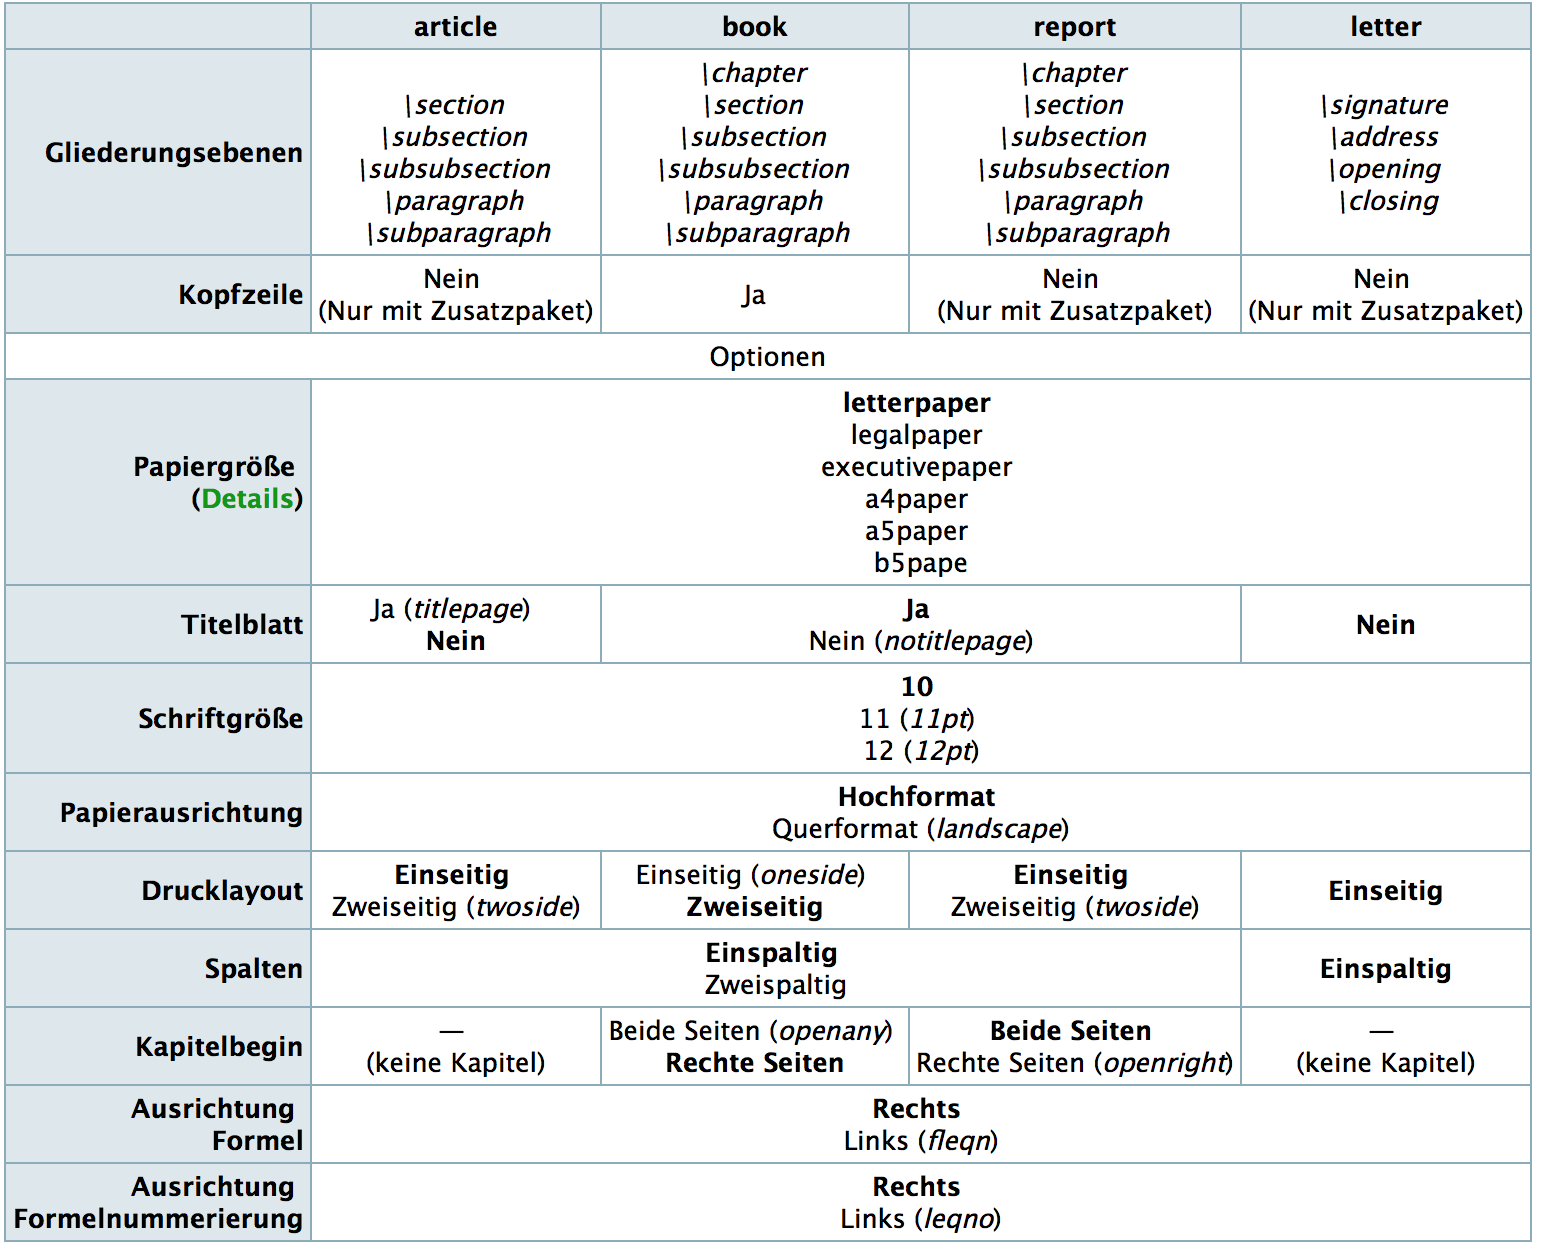
\includegraphics[width=1\textwidth]{Material/04_Dokumentenklassen.png}
		\end{figure}
	\item KOMA-Klassen
		\begin{itemize}
		\item \textbf{scrartcl}  (eine Klasse für Artikel und ähnliche Texte; diese Klasse stellt u. a. alle Optionen, Befehle und Umgebungen der Standardklasse article zur Verfügung und kann diese damit direkt ersetzen; die Anleitung findet sich in der KOMA-Script-Anleitung.)
		\item scrbook (eine Klasse für Bücher und ähnliche Texte; diese Klasse stellt u. a. alle Optionen, Befehle und Umgebungen der Standardklasse book zur Verfügung und kann diese damit direkt ersetzen; die Anleitung findet sich in der KOMA-Script-Anleitung.)
		\item \textbf{scrdoc} (eine interne, nicht dokumentierte Klasse, die für die Implementierungsdoku der KOMA-Script-Quellen und die Doku einiger Alpha- und Beta-Pakete in KOMA-Script verwendet wird.)
		\item scrlettr (ist eine obsolete Briefklasse, die nicht mehr gepflegt wird, für die es keinen Support mehr gibt, und die nicht mehr verwendet werden sollte. Für die Klasse kann bei Bedarf eine eigene Anleitung aus den Quellen scrlettr.dtx erzeugt werden. Das Paket ist seit KOMA-Script 3.12 nicht mehr in KOMA-Script enthalten, sondern nur noch in KOMA-Script obsolete.)
		\item \textbf{scrlttr2} (eine Briefklasse für Briefe; diese Klasse ist nicht kompatibel mit der Standardklasse letter; zu der Klasse gehören noch diverse Dateien mit der Endung lco über die die Klasse an unterschiedliche Anforderungen angepasst wird; die Anleitung findet sich in der KOMA-Script-Anleitung.)
		\item \textbf{scrreprt} (eine Klasse für Berichte und ähnliche Texte; diese Klasse stellt u. a. alle Optionen, Befehle und Umgebungen der Standardklasse report zur Verfügung und kann diese damit direkt ersetzen; die Anleitung findet sich in der KOMA-Script-Anleitung.)
		\item \textbf{scrguide} (eine Klasse, die nur in den KOMA-Script-Quellen zu finden ist und ausschließlich dem Setzen der KOMA-Script-Anleitung dient; diese Klasse erweitert die Klasse scrbook und passt diese den besonderen Anforderungen an; es existiert keine Anleitung zu dieser Klasse.)
		\end{itemize}
	\end{enumerate}
	
\item Gliederungsbefehle (\verb|part|, \verb|chapter|, \verb|section|, \verb|subsection|, \verb|subsubsection|, \verb|paragraph| und \verb|subparagraph|)
	\begin{enumerate}
		\item Gliederungsbefehle strukturieren Dokumente
		\item Ermöglichen automatische Nummerierungen, Eintragungen in Verzeichnisse (z.B. Inhaltsverzeichnis)
		\item Verwendbarkeit hängt von Dokumentenklasse ab.
	\end{enumerate}	

\item Shortcuts Texworks erklären

\item \textbf{Aufgabe: } Erstelle ein \LaTeX -Dokument, in dem verschiedene Gliederungselemente vorkommen. Finde heraus, welche in welcher Dokumentenklasse funktionieren. Dafür habe ich ein Template vorbereitet.
\end{enumerate}
\end{document}
